\begin{frame}{RISC-V introduction}
  \begin{itemize}
     \item Open standard instruction set architecture (ISA)
     \item Reduced instruction set computer (RISC)
     \item Designed by University of California, Berkeley. 
     \item Industry relevant:
       \begin{itemize}
         \item European Processor Initiative (EPI): RISC-V based European processor.
       \end{itemize}
  \end{itemize}
\end{frame}

\begin{frame}{RISC-V ISA details}
  \begin{itemize}
     \item Implements privileged and unprivileged ISA.
     \item 32 general purpose registers (16 in embedded)
     \item Minimal instruction set required. Extensions provide additional functionality:
       \begin{itemize}
         \item \textbf{M:} Multiplication
         \item \textbf{A:} Atomics
         \item \textbf{F, D, Q:} Floating point in 32, 64 and 128 bit respectively.
         \item \textbf{Zicsr:} Control and status register support.
         \item \textbf{Zifencei:} Load/Store fence
         \item \textbf{C:} Compressed instructions.
       \end{itemize}
  \end{itemize}
\end{frame}

\begin{frame}{RISC-V: Ariane}
  \column{0.5\textwidth} % Left column and width

\begin{itemize}
    \item Ariane is a 6-stage in-order CPU
    \item Implements privilege levels M, S, U to fully support a Unix-like operating system
    \item 
\end{itemize}
\column{.5\textwidth} % Right column and width

\begin{figure}[!ht]
    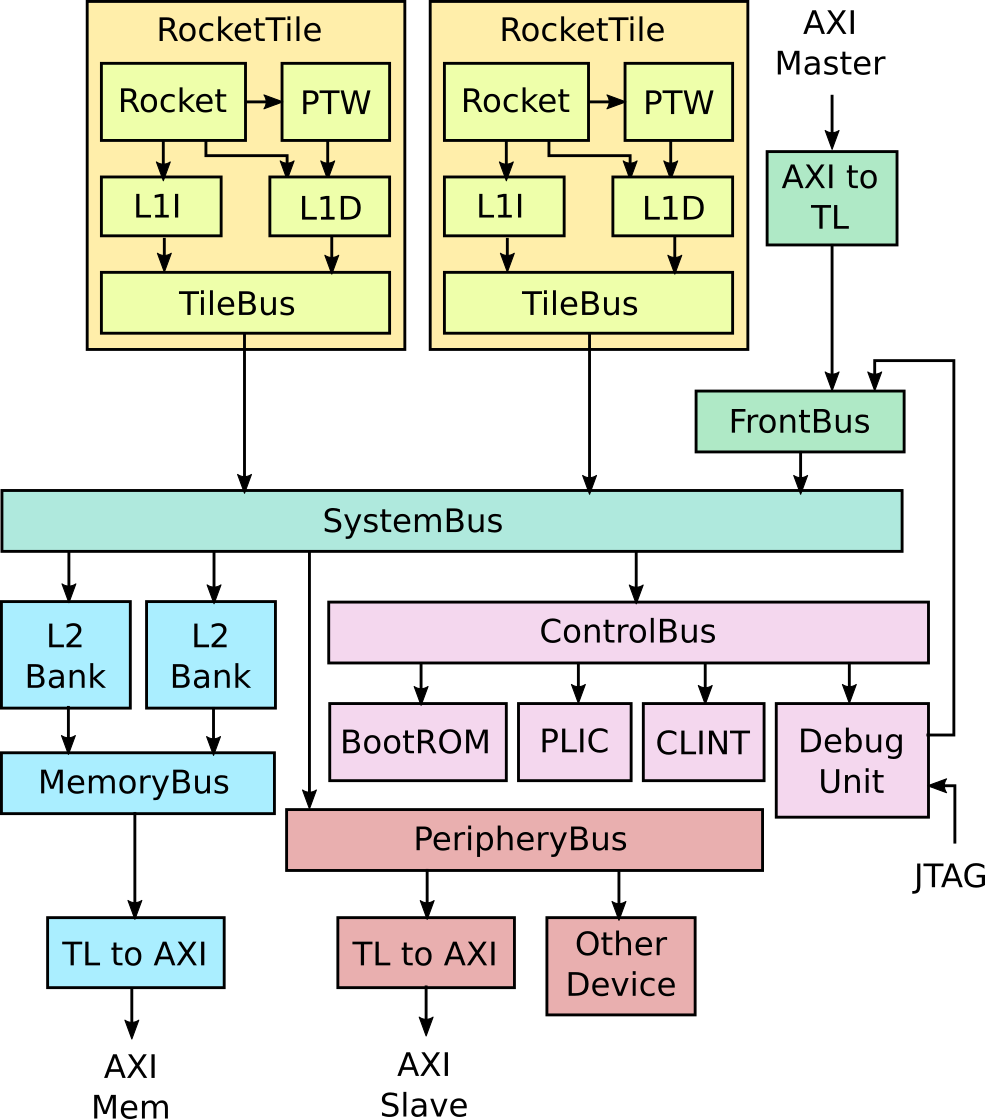
\includegraphics[width=1\linewidth]{images/rocketchip-diagram.jpg}
\end{figure}
\end{columns}
\end{frame}


\begin{frame}{RISC-V: Rocket Chip}
  \column{0.5\textwidth} % Left column and width
Rocket Chip is a SoC generator for Rocket Cores
\begin{itemize}
    \item Developed in Berkley, EEUU
    \item Hardware generation is done using Chisel
    \item Rocket core: 
    \begin{itemize}
        \item In-order scalar processor with 5-stage pipeline
        \item RV64G variant of the RISC-V ISA
    \end{itemize}
\end{itemize}
\column{.5\textwidth} % Right column and width

\begin{figure}[!ht]
    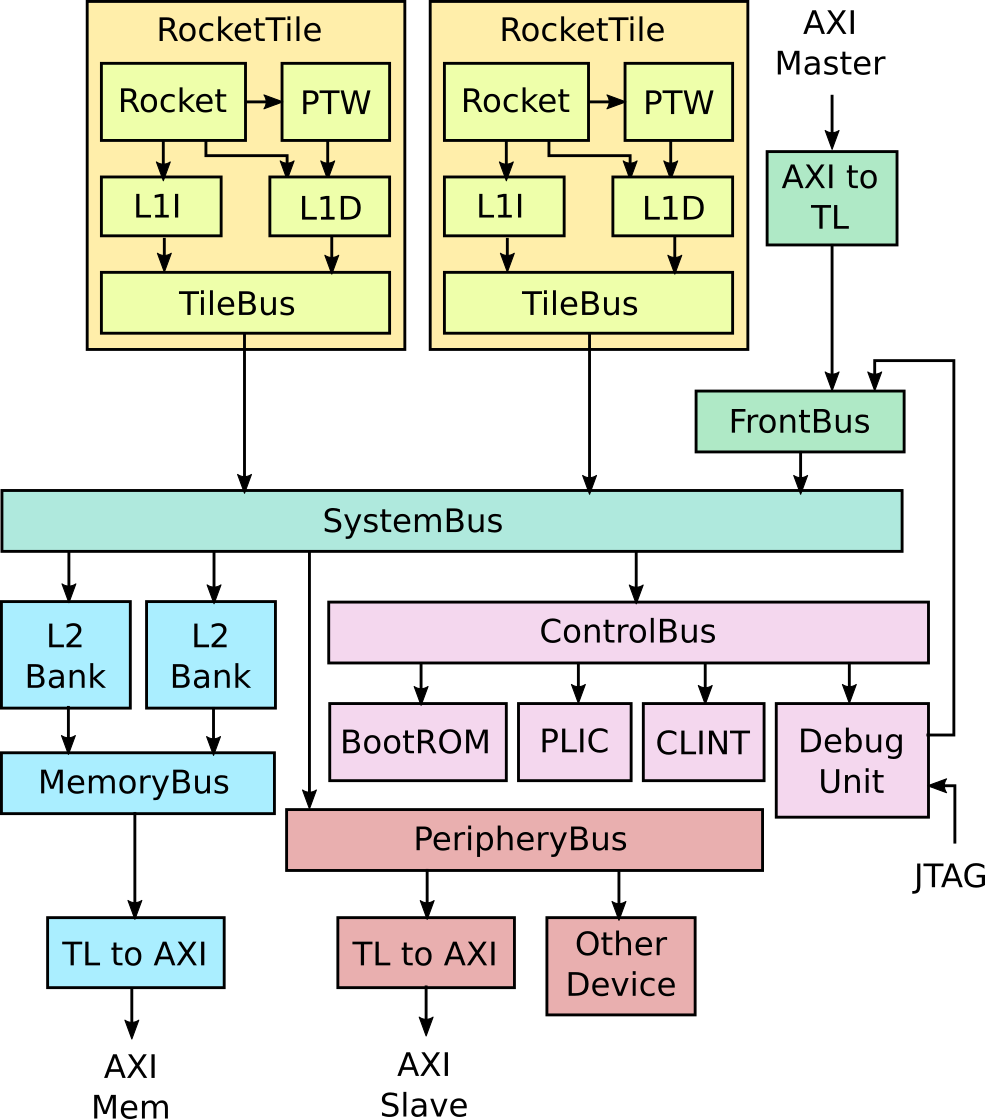
\includegraphics[width=1\linewidth]{images/rocketchip-diagram.jpg}
\end{figure}
\end{columns}
\end{frame}

